\section{Техническое предложение}
\subsection{Поиск информации о датчиках выбранного типа действия}

Потенциометрический датчик представляет собой переменный резистор, к которому приложено напряжение.
Выходная величина - разность потенциалов между подвижным контактом и одним из выходов резистора.
Она изменяется в зависимости от линейного или углового перемещения подвижного контакта.

\begin{figure}[!h]
    \centering
    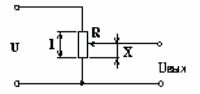
\includegraphics[width=0.5\textwidth]{img/img_1}
    \caption{Электрическая принципиальная схема потенциометрического датчика}
    \label{fig:img_1}
\end{figure}

Потенциометрические датчики по способу выполнения сопротивления делятся на три вида:
\begin{itemize}

    \item Ламельные.

    Используются для проведения относительно грубых измерений.
    Представляют из себя набор постоянных резисторов, подобранных по номиналу и припаянных к ламелям.
    Подвижный токосъемный контакт переключается между выходами резисторов, тем самым ступенчато изменяя параметры делителя напряжения.

    \begin{figure}[!h]
        \centering
        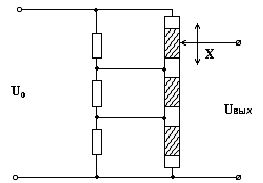
\includegraphics[width=0.5\textwidth]{img/img_2}
        \caption{Ламельный потенциометрический датчик}
        \label{fig:img_2}
    \end{figure}

    Такой тип датчика не подходит для разрабатываемого устройства ввиду низкой точности измерения.

    \item Проволочные с непрерывной намоткой.

    Датчики предназначены для более точных измерений, нежели предыдущий вариант.
    Обычно конструкционно состоят из диэлектрического материала (текстолита, гетинакса, керамики), на который в один слой намотана токопроводящая проволока с высоким удельным сопротивлением (вольфрам, манганин, фехраль).
    Токосъемый контакт, выполненный из более мягкого металла, скользит по зачищенной поверхности проволоки, намотанной на каркас, чем (аналогично предыдущему случаю) изменяет параметры делителя напряжения.

    Класс точности таких датчиком зависит от толщины проволоки и качества исполнения токосъемного контакта.
    \item С резистивным слоем.

    В датчиках с резистивным слоем вместо проволоки, намотанной на каркас, используется плоская пластина с нанесенным на нее резистивным слоем.
    Проводящий слой наносится напылением или химическим способом.
    Подвижный контакт, так же как в проволочном переменном резисторе, передвигается вдоль пластины.

    В отличие от проволочных потенциометров, точность потенциометров с резистивным слоем не зависит от диаметра используемой проволоки ввиду ее отсутствия.
    Здесь точность определяется точность нанесения резистивного слоя и качеством изготовления подвижного контакта.

\end{itemize}

С учетом описанных преимуществ и недостатков в разрабатываемом устройстве решено использовать потенциометр с резистивным слоем.
Такое исполнение является наиболее точным, а так же датчики и использованием резистивного слоя наиболее компактны.

\subsection{Разработка функциональной схемы устройства}

\begin{figure}[!h]
    \centering
    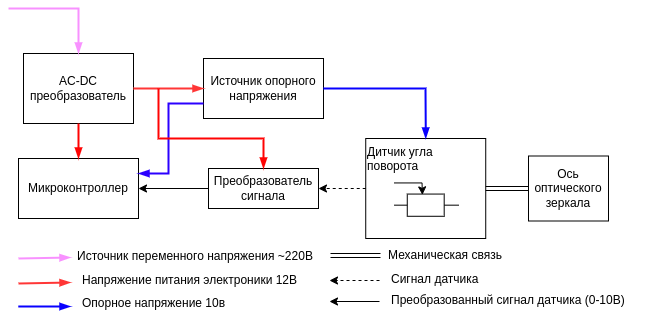
\includegraphics[width=0.9\textwidth]{img/ПИ.drawio}
    \caption{Функциональная схема измерительного устройства и его подключения к микроконтроллеру}
    \label{fig:drawio}
\end{figure}

Система питания устройства состоит из:
\begin{itemize}
    \item Источника переменного тока напряжением 220В;
    \item AC-DC преобразователя (источника постоянного напряжения 12В);
    \item Источника опорного напряжения 10В, в качестве которого может использоваться линейный стабилизатор напряжения;
    \item Используется для устранения погрешностей измерения, связанных с пульсациями в источнике питания.
\end{itemize}

Система измерения состоит из
\begin{itemize}
    \item Потенциометрического датчика углового положения, жестко связанного механически с осью зеркала(см задание);
    \item Преобразователя сигнала, масштабирующего и перемещающего выходной сигнал в требуемый диапазон (0-10В).
    Реализация планируется с использованием операционного усилителя и будет описано в следующей части.
\end{itemize}
\newpage
